\section{Procedimentos}
	Esta seção tem como objetivo relatar os procedimentos gerais da programação, por exemplo como ligar o robô, quais as funcionalidades que temos e como podemos modifica-las entre outros procedimentos.
	
	\subsection{Ligar os motores}
		Primeiramente devemos verificar se os motores estão com energia, para isso basta apenas conectar a bateria e colocar o botão de emergência na posição ON. Caso o motor esteja alimentado de forma correta, os LED's deles deverão acender e em seguida desligar. Caso isso não ocorra solicitar ajuda para a equipe de Elétrica.
		
		Com os motores alimentados (certifique-se de que o código está compilado) podemos então executar o nó dos motores de duas formas, sendo a primeira executando o comando \textit{motors} no terminal:
		
		\begin{figure}[H]
			\centering
			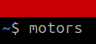
\includegraphics[scale=1]{sections/programacao/procedimentos/imagens/comando_motors.png}
		\end{figure}
		
	
		Ou indo até o diretório do RoboFEI e executando o comando \textit{source install/setup.bash} e na sequência o launch:
		
		\begin{figure}[H]
			\centering
			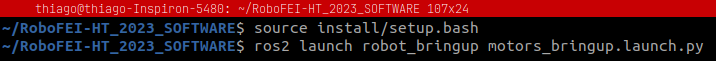
\includegraphics[scale=0.6]{sections/programacao/procedimentos/imagens/launch_motors.png}
		\end{figure}				
		
		
	\subsection{USB Rules}
		Como utilizamos mais de uma porta USB, uma para os motores e outra para a IMU foi necessário encontrarmos uma maneira de separar os USB's. Outro problema também que encontramos é que quando ligamos o USB o sistema do Linux não nos concede automaticamente permissão o suficiente para fazermos certas coisas, como por exemplo quando vamos executar o código dos motores, caso não seja dado permissão antes o código não consegue comunicar com os motores.
		
		Para tal problema podemos utilizar "Regras" para as USB, dessa forma podendo atribuir novos nomes e definir novas permissões, esse arquivo está contido no diretório do RoboFEI dentro de robot\_commands.
		
		\todo{Continuar}

\subsection{Servidor UDP}
FAZER

\subsection{Conectar Wi-Fi}
FAZER
